%%%%%%%%%%%%%%%%%%%%%%%%%%%%%%%%%%%%%%%%
% datoteka diploma-vzorec.tex
%
% vzorčna datoteka za pisanje diplomskega dela v formatu LaTeX
% na UL Fakulteti za računalništvo in informatiko
%
% vkup spravil Gašper Fijavž, december 2010
% množica popravkov v januarju, februarju marcu 2011
% verzija 29. marec 2011

\documentclass[a4paper, 12pt]{book}

\usepackage[utf8x]{inputenc}   % omogoča uporabo slovenskih črk kodiranih v formatu UTF-8 
\usepackage{hyperref}
\usepackage[slovene,english]{babel}    % naloži, med drugim, slovenske delilne vzorcecd
\usepackage[pdftex]{graphicx}  % omogoča vlaganje slik različnih formatov 
\usepackage{fancyhdr}          % poskrbi, na primer, za glave strani
\usepackage{amssymb}           % dodatni simboli
\usepackage{amsmath}           % eqref, npr.
\usepackage{inconsolata}
\usepackage{emptypage}


\renewcommand{\baselinestretch}{1.3} % ustrezen razmik med vrsticami

%oznake strani
\renewcommand{\chaptermark}[1]%
{\markboth{\MakeUppercase{\thechapter.\ #1}}{}} \renewcommand{\sectionmark}[1]%
{\markright{\MakeUppercase{\thesection.\ #1}}} \renewcommand{\headrulewidth}{0.5pt} \renewcommand{\footrulewidth}{0pt} 
\fancyhf{}
\fancyhead[LE,RO]{\sl \thepage} \fancyhead[LO]{\sl \rightmark} \fancyhead[RE]{\sl \leftmark}

\newcommand{\BibTeX}{{\sc Bib}\TeX}

\newcommand{\autfont}{\Large}
\newcommand{\titfont}{\LARGE\bf}
\newcommand{\clearemptydoublepage}{\newpage{\pagestyle{empty}\cleardoublepage}}
\setcounter{tocdepth}{1}	      % globina kazala

% konstrukti
\newtheorem{izrek}{Izrek}[chapter]
%\newtheorem{trditev}{Trditev}[izrek]
\newenvironment{dokaz}{\emph{Dokaz.}\ }{\hspace{\fill}{$\Box$}}

\begin{document}
\selectlanguage{slovene}
\frontmatter
\setcounter{page}{1} %
\renewcommand{\thepage}{}       % preprecimo težave s številkami strani v kazalu 

%%%%%%%%%%%%%%%%%%%%%%%%%%%%%%%%%%%%%%%%
%naslovnica
 \thispagestyle{empty}%
   \begin{center}
    {\large\sc Univerza v Ljubljani\\%
      Fakulteta za računalništvo in informatiko}%
    \vskip 10em%
    {\autfont Miha Zidar \par}%
    {\titfont Dostop do podatkov Svetovne banke v orodju Orange \par}%
    {\vskip 2em \textsc{DIPLOMSKO DELO\\[2mm] 
    UNIVERZITETNI ŠTUDIJSKI PROGRAM RAČUNALNIŠTVO IN INFORMATIKA}\par}%
    \vfill\null%
    {\large \textsc{Mentor}: prof. dr. Bla"z Zupan \par}%
    {\vskip 2em \large Ljubljana, 2016 \par}%
\end{center}
% prazna stran
\clearemptydoublepage

%%%%%%%%%%%%%%%%%%%%%%%%%%%%%%%%%%%%%%%%
%copyright stran
\thispagestyle{empty}
\vspace*{8cm}
{\small \noindent
Rezultati diplomskega dela so intelektualna lastnina avtorja in Fakultete za ra\-čunalništvo in informatiko Univerze v Ljubljani. 
Za objavljanje ali izkoriščanje rezultatov di\-plom\-ske\-ga dela je potrebno pisno soglasje avtorja, Fakultete za ra\-ču\-nal\-niš\-tvo in 
informatiko ter mentorja.}



\begin{center} 
\mbox{}\vfill
\emph{Besedilo je oblikovano z urejevalnikom besedil \LaTeX.} 
\end{center}
% prazna stran
\clearemptydoublepage

%%%%%%%%%%%%%%%%%%%%%%%%%%%%%%%%%%%%%%%%
% stran 3 med uvodnimi listi
\noindent
Namesto te strani {\bf vstavite} original izdane teme diplomskega 
dela s podpisom mentorja in dekana ter žigom fakultete, ki ga diplomant
dvigne v študent\-skem referatu, preden odda izdelek v vezavo!

% prazna stran
\clearemptydoublepage

%%%%%%%%%%%%%%%%%%%%%%%%%%%%%%%%%%%%%%%%
% izjava o avtorstvu
\vspace*{1cm}
\begin{center} 
{\Large \textbf{\sc Izjava o avtorstvu diplomskega dela}}
\end{center}

\vspace{1cm}
\noindent Spodaj podpisani Miha Zidar,
z vpisno številko \textbf{63060317}, sem avtor  diplomskega dela z naslovom:
   
\vspace{0.5cm}
\emph{Dostop do podatkov Svetovne banke v orodju Orange}

\vspace{1.5cm}
\noindent S svojim podpisom zagotavljam, da:
\begin{itemize}
	\item sem diplomsko delo izdelal samostojno pod mentorstvom 
        prof.\ dr.\ Bla"za Zupana,

	\item so elektronska oblika diplomskega dela, naslov (slov., angl.), povzetek (slov., angl.) ter ključne besede (slov., angl.) identični s tiskano obliko diplomskega dela
	\item soglašam z javno objavo elektronske oblike diplomskega dela v zbirki ''Dela FRI''.
\end{itemize}

\vspace{1cm}
\selectlanguage{slovene}
\noindent V Ljubljani, dne \today \hfill Podpis avtorja:

% prazna stran
\clearemptydoublepage

%%%%%%%%%%%%%%%%%%%%%%%%%%%%%%%%%%%%%%%%
% zahvala
\thispagestyle{empty}\mbox{}\vfill\null\it%
Zahvalil bi se mentorju, prof.\ dr.\ Bla"za Zupana, za pomoč in usmerjanje med izdelavo diplomskega dela. Prav tako bi se za spodbudo zahvalil svojim staršem in prijateljem.
\rm\normalfont

% prazna stran
\clearemptydoublepage

%%%%%%%%%%%%%%%%%%%%%%%%%%%%%%%%%%%%%%%%
% posvetilo
\thispagestyle{empty}\mbox{}{\vskip0.20\textheight}\mbox{}\hfill\begin{minipage}{0.55\textwidth}%
    % bubi
\normalfont\end{minipage}
 
% prazna stran
\clearemptydoublepage

%%%%%%%%%%%%%%%%%%%%%%%%%%%%%%%%%%%%%%%%
% kazalo
\def\thepage{}% preprecimo tezave s stevilkami strani v kazalu 
\tableofcontents{}


% prazna stran
\clearemptydoublepage

%%%%%%%%%%%%%%%%%%%%%%%%%%%%%%%%%%%%%%%%
% povzetek 
\addcontentsline{toc}{chapter}{Povzetek}
\chapter*{Povzetek}


\textbf{Naslov:} Dostop do podatkov Svetovne banke v orodju Orange

\ \\
\textbf{Avtor:} Miha Zidar

\ \\
% TODO dodaj kaksen stavek ali dva
Program Orange je orodje za podatkovno rudarjenje, v katerem
lahko za namene analiz uporabimo razli"cne podatkovne vire. Sam program Orange
vsebuje predpripravljene zbirke podatkov, dodatne zbirke podatkov si lahko 
pripravi in uvozi tudi uporabnik sam, ali pa uporabi katerega od "ze obstoje"cih
dodatkov za uvoz podatkov. Za namen diplomske naloge smo izdelali dodatek 
Orange data sets, s katerim je mogo"ce dostopati do podatkov s programskega 
vmesnika Svetovne banke. Trenutno Svetovna banka omogo"ca uporabo "stirih 
razlicnih programskih vmesnikov: gospodarski indikatorji, projekti Svetovne banke, 
finan"cni podatke in klimatski podatki. Dodatek Orange data sets vsebuje dva
gradnika, ki sta namenjena la"zjemu branju in uporabi podatkov indikatorjev in 
klimatskih podatkov.
S tem bo uporabnikom programa Orange omogo"cena enostavnej"sa uporaba velikega "stevila
podatkov iz omenjenih dveh programskih vmesnikov.

\ \\
\textbf{Klju"cne besede:} Podatkovno rudarjenje, programski vmesnik, 
Svetovna banka, gospodarski indikatorji, podnebni podatki, Orange. 




% prazna stran
\clearemptydoublepage

%%%%%%%%%%%%%%%%%%%%%%%%%%%%%%%%%%%%%%%%
% abstract
\selectlanguage{english}
\addcontentsline{toc}{chapter}{Abstract}
\chapter*{Abstract}


\textbf{Title:} Access to World bank data with Orange

\ \\
\textbf{Author:} Miha Zidar

\ \\
TODO: Orange is an open source data-mining software, capable of using multiple
sources for data analysis. There are a few test data sample already present
in Orange, and the user can import their own data sets with the use of one of
Orange input widgets. For this thesis we created a new widget "Orange data sets"
for accessing free data from World bank application program interface (API).
The World bank exposes four different data APIs; indicator, project, finance
and climate. Our Orange data sets widget will be able to read data from the
indicators and climate APIs.


\ \\
\textbf{Key words:} Data mining, API, World bank, indicators, climate, Orange.

\selectlanguage{slovene}


\selectlanguage{slovene}
% prazna stran
\clearemptydoublepage

%%%%%%%%%%%%%%%%%%%%%%%%%%%%%%%%%%%%%%%%
\mainmatter
\setcounter{page}{1}
\pagestyle{fancy}



\chapter{Uvod}

Na spletu je vedno ve"c prosto dostopnih programskih vmesnikov za razne
baze podatkov. Te vmesniki ponujajo dostop do zelo raznolikih podatkov, kot so 
seznami stopnje ogro"zenosti "zivali po dr"zavah 
\fnurl{http://apiv3.iucnredlist.org/api/v3/docs}, 
NASA podatki meritev in slike vesolja 
\fnurl{https://api.nasa.gov/}, 
seznam knjig z ocenami in povezavami med uporabniki 
\fnurl{https://www.goodreads.com/api},
zgodovina meteorolo"skih meritev
\fnurl{http://climatedataapi.worldbank.org/}, 
razni indikatorji stopnje razvoja dr"zav
\fnurl{http://api.worldbank.org/}.

Ker pa so programski vmesniki bolj splo"sno namenski, je
podatke te"sko spraviti v obliko ki bi bila primerna za uporabo v raznih 
orodjih za analizo in obdelavo podatkov. Prav tako se ve"cina programov in knji"znic za dostop
do baz podatkov osredoto"ci le na iskanje po teh bazah, ne pa tudi na
pridobivanje "cim ve"cje koli"cine podatkov.


% Poleg tega obstaja dosti odprto kodnih programov za obdelavo 
% in analizo podatkov. Ker so programski vmesnike bolj splo"sno namenski, je
% podatke te"sko spraviti v obliko za analizo in obdelavo. Z orodjem, ki bi
% pomagalo zdru"ziti programe za obdelavo podatkov in prosto dostopne baze
% podatkov, bi omogo"cili raziskovanje teh podatkov "sir"si javnosti.



% Povezava programskega vmesnika in orodja za analizo podatkov pa je pogosto 
% prezapletena za navadnega uporabnika. Z dodajanjem gradnikov za enostavno 
% uporabo spletnih programskih vmesnikov v orodjih kot je Orange, omogo"cimo ...

\section{Motivacija}

Branje podatkov z raznih programskih vmesnikov je lahko zelo zamudno delo.
Programski vmesnik se lahko s "casom spremeni, in podatki ki jih dobimo z
vmesnika so lahko pokvarjeni. Trenutni pristop, kjer moramo podatke vsaki"c ro"cno
obilkovati da so primerni za analizo, ima mnogo pomanjkljivosti. Prejeti podatki
lahko vsebujejo nepravilnosti, ali pa so celo nedostopni. Z dodatkom ki bi
poskrbel za prenos podatkov in pretovrbo v uporabno obliko, hkrati pa bi znal
popraviti ali odstraniti pokvarjene podatke, bi lahko ve"c pozornosti posvetili
sami analizi in obdelavi. Poleg tega, pa ve"cina knji"znic za delo z odprtimi
programskimi vmesniki, nudi zelo dobre na"cine za iskanje posameznih podatkov,
ne pa za prenos ve"cje koli"cine podatkov kar je bolj primerno za analizo in
obdelavo.



\section{Cilji}

Cilj diplomske naloge je izdelati knji"znico, ki omogo"ca enostaven dostop do
podatkov Svetovne banke in interaktivni gradnik v programu Orange za dostop in
uporabo teh podatkov. S tem bomo omogo"cili raziskovanje teh podtakov "sir"si
javnosti. Knji"znica bo poenostavila prenos ve"cjega "stevila podatkov, in
predstavila te podatke v obliki primerni za orodje Orange. k<

\chapter{Spletni viri indikatorjev drzav sveta}

Na spletu je mnogo prosto dostopnih virov oz. baz podatkov. Ti imajo programske
vmesnike, ki omogocajo dostop do raznovrstnih podatkov, kot so npr. seznami 
stopnje ogrozenosti zivali po drzavah 
\fnurl{http://apiv3.iucnredlist.org/api/v3/docs},
Nasini podatki meritev in slike vesolja
\fnurl{https://api.nasa.gov/}
seznam knjig z ocenami in povezavami med uporabniki
\fnurl{https://www.goodreads.com/api},
zgodovina meteoroloskih meritev
\fnurl{http://climatedataapi.worldbank.org/},
razni indikatorji stopnje razvoja drzav
\fnurl{http://api.worldbank.org/}.
Pri nalogi smo se osredotocili na dva programska vmesnika za dostop podatkov 
Svetovne banke, to sta zgodovina meteoroloskih meritev (4) in razni 
indikatorji stopnje razvoja drzav (5).


% 1 IUCN 2016. IUCN Red List of Threatened Species. Version 2016-1 <www.iucnredlist.org>
% http://apiv3.iucnredlist.org/api/v3/docs
% 
% 2 https://api.nasa.gov/#getting-started
% 
% 3 https://www.goodreads.com/api
% 
% 4 http://climatedataapi.worldbank.org/
% 
% 5 http://api.worldbank.org/


Za podatkovno bazo Svetovno banko smo se odlocili, ker zdruzuje in na enovit
nacin predstavi podatke iz vec razlicnih virov. Podatkovni viri za indikatorje
stopnje razvoja drzav so:

- World Development Indicators, 
- Global Development Finance, 
- African development Indicators, 
- Doing Business,
- Enterprise Surveys, 
- Millennium Development Goals, 
- Education Statistics, 
- Gender Statistics,
- Health and Nutrition Statistics, 
- IDA Results Measurement System.

Podatkovni viri za klimatske meritve so pridobljeni s svetovnih meteoroloskih 
postaj.


Dostop do podatkov je omogocen prek vmesnika REST, ki ponuja veliko moznosti 
za iskanje in presejanje rezultatov. 


Note: vse zahteve so omejene s kolicino podatkov na stran in za dostop do vseh
se moramo sami sprehoditi cez vse strani.

format zahtev:

\begin{lstlisting}
[

    {
        "page": 1,
        "pages": 6,
        "per\_page": "2000",
        "total": 304
    },
    [
        {<podatki>}
	]
]
\end{lstlisting}





\section{Podatki indikatorjev razvoja drzav}

Programski vmesnik indikatorjev razvoja drzav Svetovne banke omogoca dostop
do prek 16.000 raznih indikatorjev. Podatki indikatorjev so merjeni od leta
1960 dalje v mesecnem, cetrtletnem ali letnem intervalu. 


Za dostop do podatkov posameznega indikatorja, potrebujemo identifikator (id)
indikatorja in kodo drzave ali regije. 


\subsection{Opis programskega vmesnika indikatorjev}
Seznam vseh indikatorjev z imeni, opisi, in identifikatorji lahko dobimo na 
naslovu http://api.worldbank.org/indicators.

\ \\
Primer podatkov indikatorja "Poverty Headcount (\$2.50 a day)" (stopnja revscine
pri dohodku 2,5 dolarja na dan) v obliki JSON.

\begin{lstlisting}
{
    "id": "1.0.HCount.2.5usd",
    "name": "Poverty Headcount (\$2.50 a day)",
    "source": {
        "id": "37",
        "value": "LAC Equity Lab"
    },
    "sourceNote": "The poverty headcount index measures the proportion of the 
                   population with daily per capita income (in 2005 PPP) below
                   the poverty line.",
    "sourceOrganization": "LAC Equity Lab tabulations of SEDLAC (CEDLAS and the
                           World Bank).",
    "topics": [
        {
            "id": "11",
            "value": "Poverty "
        }
    ]
}
\end{lstlisting}


\subsection{Opis programskega vmesnika drzav}
Seznam kod drzav in regij se nahaja na naslovu 
http://api.worldbank.org/countries.

Primer

\begin{lstlisting}
{
    "id": "ABW",
    "iso2Code": "AW",
    "name": "Aruba",
    "region": {
        "id": "LCN",
        "value": "Latin America & Caribbean "
    },
    "adminregion": {
        "id": "",
        "value": ""
    },
    "incomeLevel": {
        "id": "HIC",
        "value": "High income"
    },
    "lendingType": {
        "id": "LNX",
        "value": "Not classified"
    },
    "capitalCity": "Oranjestad",
    "longitude": "-70.0167",
    "latitude": "12.5167"
},
\end{lstlisting}

Kode drzav, ki jih lahko uporabimo v poizvedbah, ustrezajo standardu ISO 
3166-1 \fnurl{http://www.iso.org/iso/country_codes.htm} 
alpha-2 ali ISO 3166-1 alpha-3.
Poleg tega gornji seznam drzav vsebuje tudi dodatne kode za agregate, kot so:
- regije
- skupine drzav po visini dohodka
- nekatere izjeme drzav, kot je trenutno Kosovo.



\subsection{Dostop do podatkov indikatorjev}
Dostop do podatkov posameznega indikatorja je mogoc na naslovu
http://api.worldbank.org/countries/<country\_list>/indicators/<indicator\_id>,
kjer je:

- country\_list; z podpicjem locen seznam kod drzav, ki jih dobimo v polju "id"
ali "iso2Code" v zgoraj opisanem seznamu drzav,
- indicator\_id; identifikacijska koda (id) indikatorja.


Izsek podatkov:
\begin{lstlisting}
...
{

    "indicator": {
        "id": "SP.POP.TOTL",
        "value": "Population, total"
    },
    "country": {
        "id": "IL",
        "value": "Israel"
    },
    "value": "6289000",
    "decimal": "0",
    "date": "2000"
},
{
    "indicator": {
        "id": "SP.POP.TOTL",
        "value": "Population, total"
    },
    "country": {
        "id": "IT",
        "value": "Italy"
    },
    "value": "56974100",
    "decimal": "0",
    "date": "2001"

},
...
\end{lstlisting}


Vmesnik indikatorjev SB omogoca poizvedbe z naslednjimi parametri:

\begin{itemize}  
\item MRV (most rescent value) - nekaj zadnjih meritev
\item frequency - pogostost vzorcenja (letno, cetrtletno, mesecno)
\item gapfill - manjkajoce vrednosti prejsnjih meritev
\item date - datum ali obdobje
\item page - stran
\item per\_page - stevilo elementov na stran
\end{itemize}






\section{Tezave pri dostopu}


Tezave pri uporabi SB API-ja lahko razdelimo v dve skupini. Prva skupino
sestavljajo tezave pri dokumentaciji in z manjkajocimi podatki, drugo pa
napake v samih pridobljenih podatkih.

Tezave prve skupine:

- ob posodabljanju spletne strani SB se izgubijo posamezne povezave do 
  primerov, dokumentacije in opisov API-ja,
- nepopolna dokumentacija:
  - polje za datum je opisano, vendar ni dokumentirano, kaksne so vse mozne 
    vrednosti,
  - delovanje polj za obdobje (date), zadnje vrednosti (mrv) in za mankjajoce
    vrednosti (gapfill) ni ustrezno opisano.

Tezave druge skupine:


- manjkajoci identifikatoriji za polja na posameznih indikatorjih (primer je
  manjkajoca vrednost v polju id drzave),
- datum vsebuje nakljucne vrednosti ("last known value", "2001 - 2015", "2040"),
- zgornja meja stevila izbranih lokacij na 250 ni navedena,
- nemogoce je ugotoviti pogostost vzorcenja indikatorja (frequency).





CCCCC


\chapter{Knjižnica in gradniki za Orange}

V okviru diplomske naloge smo razvili tri ločene komponente za programerje in
končne uporabnike programa Orange. Prva komponenta je
dostopna kot samostojni paket 
\verb|simple_wbd|\fnurl{https://pypi.python.org/pypi/simple_wbd/0.5.0}. 
Druga in tretja komponenti pa sta združeni v paketu
\verb|orange3-datasets|\fnurl{https://pypi.python.org/pypi/Orange3-Datasets/0.1.3}

Prva komponenta je programska knjižnica \verb|simple_wbd|, ki
omogoča enostaven dostop do programskega vmesnika indikatorjev in podnebnih
podatkov Svetovne banke. Ta knjižnica je narejena s čim manj odvisnosti in je 
% TODO ali je python z veliko
namenjena splošni uporabi v Python programih. Poudarka pri zasnovi knjižnice 
\verb|simple_wbd| sta predvsem enostavnost razširitve in zanesljivost. Ta cilja
dosežemo z mehanizmom za vključevanje lastne kode v komponente knjižnice
in mehanizmi za popravljanje ali odstranjevanje pokvarjenih podatkov.

Drugi sestavni del je razširitev knjižnice \verb|simple_wbd| s 
funkcionalnostmi, potrebnimi za lažje delo v programu Orange. To predvsem 
zavzema pretvorbo pridobljenih podatkov v podatkovno tabelo Orange in tabelo 
numpy. Ta sklop je namenjen skriptnemu delu s programom Orange 
\cite{orange_scripting} in je dostopen
kot \verb|api_wrapper| Python modul znotraj paketa \verb|orangecontrib.wbd|.

Tretji sestavni del je grafični vmesnik za uporabo \verb|api_wrapper| modula.
Namen grafičnega vmesnika je omogočiti ne-programerjem dostop do podatkov 
programskega vmesnika Svetovne banke znotraj programa Orange za namen obdelave,
analize in iskanja zakonitosti v podatkih.

\section{Knjižnica simple\_wbd}

Knjižnica \verb|simple_wbd| programerjem olajša dostop do podatkov 
programskega vmesnika Svetovne banke. Glavna lastnost te knjižnice je 
združevanje večjega števila zahtev po podatkih in enostavna predstavitev 
prejetih podatkov. Druga lastnost je pretvorba podatkov iz več dimenzij v 
dvo-dimenzionalno polje, primerno za uporabo v programu Orange. Glavna 
razreda te knjižnice sta \verb|IndicatorAPI| in \verb|ClimateAPI|. Prvi 
omogoča pridobivanje podatkov iz programskega vmesnika indikatorjev, drugi pa 
s programskega vmesnika podnebnih meritev.


Čeprav za dostop do programskega vmesnika Svetovne banke že obstajajo 
rešitve kot sta knjižnici 
\verb|wbdata|\fnurl{https://pypi.python.org/pypi/wbdata} in
\verb|wbpy|\fnurl{https://pypi.python.org/pypi/wbpy/2.0.1}, smo se odločili
za lastno implementacijo podobne knjižnice. Glavni razlog za to je, da
obstoječe rešitve poskušajo čim bolj natančno predstaviti programski
vmesnik Svetovne banke, ne pa olajšati dostop do čim večje količine
podatkov.

Za potrebe te knjižnice smo razvili lastno rešitev za predpomnjenje poizvedb,
saj so se bolj splošne rešitve, kot na primer
\verb|vcrpy|\fnurl{https://pypi.python.org/pypi/vcrpy/1.10.0} in
\verb|requests-cache|\fnurl{https://pypi.python.org/pypi/requests-cache}, 
izkazale za prepočasne ko delamo z večjimi količinami podatkov. Naša
rešitev za predpomnjenje izkorišča dejstvo da je vsaka poizvedba določena le
z naslovom URL, in da so vsi odgovori oblike JSON. Za vsak URL naredimo novo
datoteko v sistemskem začasnem imeniku, v kateri hranimo serializirane JSON
podatke. Ker se podatki na programskem vmesniku Svetovne banke redko
posodabljajo, smo za čas veljavnosti začasnih datotek izbrali en teden.

% NOTE: serailizacija je baje uredu beseda:
% http://eprints.fri.uni-lj.si/2711/1/63100205-VALENTIN_KRAGELJ-\
% Pregled_in_analiza_tehnologij_za_serializacijo_objektov.pdf


\subsection{Razred IndicatorAPI}
\label{razered_indicator_api}

\verb|IndicatorAPI| je razred namenjen pridobivanju podatkov indikatorjev
razvoja držav. Ker ima programski vmesnik Svetovne banke omejitev koliko 
podatkov lahko prenesemo z eno poizvedbo in nam dovoli tvoriti poizvedbe le za
en indikator na enkrat, smo napisali razred, ki v ozadju tvori in izvede
poizvedbe za vse strani vseh zahtevanih indikatorjev. To poskrbi tako da se po
prvi poizvedbi za en indikator sprehodi čez število preostalih strani 
(Primer \ref{basic_response}), ki so na voljo, in pridobljene podatke večih
strani združi in predstavi kot rezultat ene same poizvedbe. Ta postopek ponovi
za vse zahtevane indikatorje, in njihove rezultate vrne v obliki slovarja, ki 
ima za ključ kodo indikatorja posamezne zahteve.

Poleg tega da skrbi za prenos vseh strani podatkov, tudi beleži število 
izvedenih in število potrebnih poizvedb za celoten prenos. Ta števila se
lahko uporablja za prikaz napredka prenosa podatkov.


Za namene razreda \verb|IndicatorAPI| smo v knjižnici \verb|simple_wbd|
razvili mehanizme za odpravo nekaterih napak omenjenih v poglavju 
\ref{api_gotchas}.

Pri manjkajočih vrednostih držav v poizvedbah za podatke indikatorjev,
poskušamo določiti pravilne vrednosti. To naredimo s pomočjo dveh
slovarjev: prvi slika kode držav v imena, drugi pa imena držav v kode. V
primeru manjkajoče vrednosti kode ali imena, poskušamo to prebrati iz enega
od naštetih slovarjev. Če nam ne uspe ugotoviti manjkajočih vrednosti,
trenutni vnos odstranimo iz rezultata poizvedbe.

Drugi tip napak, ki ga lahko delno popravimo, so napačne vrednosti v polju
\verb|date| v poizvedbah za podatke indikatorjev. Ker lahko v temu polju
pričakujemo poljubno besedilo, dela naš pretvornik za polje \verb|date| v 
datum, tako da poskuša v datum pretvoriti čim daljšo predpono besedila.
Če nam ne uspe besedila pretvoriti v veljaven datum, trenutni vnos odstranimo
iz rezultata poizvedbe.


\ \\
Glavne metode ki jih ponuja razred IndicatorAPI so:

\begin{description}  
\item [get\_indicators] za pridobivanje seznama indikatorjev s kodami, imeni
      in opisi,
\item [get\_countries] za pridobivanje seznama držav z metapodatki,
\item [get\_dataset] za pridobivanje instance razreda \verb|IndicatorDataset|,
      ki vsebuje podatkov indikatorjev.
\end{description}

Ena izmed lastnosti razreda \verb|IndicatorAPI| je ta da mu lahko ob
inicializaciji podamo razred v katerem želimo prejeti rezultat poizvedbe. Ta
razred mora dedovati od osnovnega razreda \verb|IndicatorDataset|. Na ta
način lahko enostavno razširimo funkcionalnost \verb|simple_wbd| knjižnice.
V primeru \ref{indicator_api_extend} vidimo en način za razširitev razreda 
\verb|IndicatorDataset| tako da uporabniku razreda \verb|MyIndicatorAPI| ni
potrebno izrecno podati razreda \verb|IndicatorDataset| v konstruktor.

\begin{snippet}
\begin{center}
\begin{lstlisting}
class MyIndicatorDataset(simple_wbd.IndicatorDataset):
    
    def as_numpy(self):
        raise NotImplemented()
    
    def as_orange_table(self):
        raise NotImplemented()

class MyIndicatorAPI(simple_wbd.IndicatorAPI):

    def __init__(self):
        super().__init__(MyIndicatorDataset)
\end{lstlisting}
\end{center}
\caption[some]{Primer razširitve osnovnega razreda rezultatov poizvedb.}
\label{indicator_api_extend}
\end{snippet} 


\subsubsection{Razred IndicatorDataset}
\label{razred_indicatordatasets}

Razred \verb|IndicatorDataset| je osnovni razred v katerem dobimo zahtevane 
podatke indikatorjev. Ta razred vsebuje vse potrebne metode in podatke za 
predstavitev rezultatov programskega vmesnika, na dva načina: kot slovar
rezultatov poizvedb za posamezen indikator in dvo dimenzionalen seznam. 
Posamezna vrednost v teh podatkih je določena z državo, časovno komponento in 
kodo indikatorja. 

Podatke lahko predstavimo kot dvodimenzionalno polje v dveh oblikah: kot
časovne vrste ali kot podatki držav. Obliko predstavitve izberemo s
parametrom \verb|time_series| metode \verb|as_list|. Za predstavitev obeh oblik
je prva vrstica polja uporabljena kot naslovna vrstica, ki opisuje podatke v 
stolpcih.

Ko uporabljavo obliko časovnih vrst, so elementi prve vrstice kartezični
produkt kod indikatorjev in držav. V prvem stolpcu polja pa imamo časovno
komponento podatkov. Na ta način so vsi ostali elementi polja določeni s 
časovno komponento, državo in kodo indikatorja.

Ko dostopamo do dvodimezionalnega polja ki predstavlja podatke držav, pa je v
prvi vrstici kartezični produkt kod indikatorjev in časovne komponente. Prvi
stolpec v tej predstavitvi vsebuje imena držav. Za razliko od predstavitve v 
obliki časovnih vrst, v to polje vstavimo se dodatne stolpce ki vsebujejo
metapodatke drzav iz primera \ref{country_response}: regija \verb|region|, 
administrativna regija \verb|adminregion|, višina dohodka \verb|incomeLevel|, 
vrsta posojil \verb|lendingType|, geografska širina \verb|latitude|, 
geografska dolžina \verb|longitude|. Tudi tukaj vsi ostali elementi določeni s
časovno komponento, državo in kodo indikatorja. 


\subsection{Razred ClimateAPI}

Razred \verb|ClimateAPI| olajša dostop do podnebnih podatkov programskega
vmesnika Svetovne banke. Ta programski vmesnik dovoli poizvedbe po podatkih le 
ene vrste meritev za eno vrsto meritvenega obdobja in eno državo. Naš razred 
naredi kartezični produkt med vsemi zahtevanimi vrstami meritev, vrstami
meritvenih obdobij in državami. Nato iz tega zgradi in izvede vse poizvedbe 
in predstavi podatke kot enotni odgovor. V razredu \verb|ClimateAPI| hranimo 
tudi število vseh potrebnih poizvedb in število že izvedenih poizvedb, kar 
lahko uporabimo za prikaz napredka prenosa podatkov.



\subsubsection{Razred ClimateDataset}

Razred \verb|ClimateDataset| je osnovni razred v katerem dobimo zahtevane 
podatke podnebnih meritev. Ta razred vsebuje vse potrebne metode in podatke za 
predstavitev rezultatov programskega vmesnika, na dva glavna načina: kot
gnezden slovar in dvo dimenzionalen seznam. Posamezna vrednost v teh podatkih
je določena z državo, vrsta podatkov, in časovno komponento. Poleg omenjenih
načinov predstavitve podatkov lahko dostopamo tudi do neobdelanih podatkov 
prejetih iz programskega vmesnika za vsako poizvedbo posebej.

Časovna komponenta rezultata je sestavljena iz vrste meritvenega obdobja in 
začetkom obdobja meritve. Sestavljajo časovno komponento uporabljamo, da se 
izognemo dvoumnim primerom vrednosti začetka obdobja za letni in desetletni 
interval meritev. Primera takih dveh časovnih obdobij sta 
\verb|'decade - 1990'| in \verb|'year - 1990'|.


Do podatkov predstavljenih z gnezdenim slovarjem lahko dostopamo preko funkcije
\verb|as_dict|. V tej funkciji združimo podatke poizvedb programskega
vmesnika v gnezden slovar s štirimi nivoji gnezdenja: država, vrsta meritev,
vrsta meritvenega obdobja in obdobje meritve. Zadnji nivo gnezdenja vsebuje
vrednosti podnebnih meritev.

Pri predstavitvi podatkov kot dvodimenzionalno polje, moramo dve od treh
komponent podatkov (država \verb|'country'|, vrsta podatkov \verb|'type'|, 
in časovna komponenta \verb|'interval'|)
združiti in ju skupaj prikazati v vrsticah ali stolpcih. Za razliko od razreda
\verb|IndicatorDataset|, ki podpira le dve obliki prikaza, lahko v razredu
\verb|ClimateDataset| sami določimo katere komponente bodo v stolpcih in
katere v vrsticah. Primer različnih izborov komponent je prikazan v
\ref{list_configurations}. Spremenljivki \verb|list1| ind \verb|list2| iz
prejšnjega primera prikazujeta privzeto konfiguracijo, kjer imamo v stolpcih
kartezični produkt vrst meritev in vrst meritvenih obdobij, v vrsticah pa
podatke države. Spremenljivka \verb|list4| prikazuje konfiguracija za
predstavitev v obliki časovnih vrst.

\begin{snippet}
\begin{center}
\begin{lstlisting}
import simple_wbd

api = simple_wbd.ClimateAPI()                   
climate_dataset = api.get_instrumental(['svn', 'usa', 'aus'])

list1 = ds.as_list()
list2 = ds.as_list(columns=['type', 'interval'])  # default  value
list3 = ds.as_list(columns=['type'])
list4 = ds.as_list(columns=['type', 'country']) 
list5 = ds.as_list(columns=['country'])
\end{lstlisting}
\end{center}
\cprotect
\caption{Prikaz nekaj možnih oblik dvodimezionalnega polja vrednosti.} 
\label{list_configurations}
\end{snippet} 



\section{Modul api\_wrapper}


Znotraj paketa \verb|orangecontrib.wbd| smo razvili modul \verb|api_wrapper| v
katerem smo razširili razreda \verb|IndicatorDataset| in \verb|ClimateDataset|
na način ki je prikazan v primeru \ref{indicator_api_extend}. Naša
razširitev obema razredoma doda metodi za pretvorbo podatkov v podatkovno 
tabelo Orange in tabelo numpy.

\subsection{Razširitev razreda IndicatorDataset}

Glavne funkcionalnosti, za uporabo programske vmesnika indikatorjev, so
vključene v naši razširitvi razreda \verb|IndicatorDataset|. To je na prvem
mestu metoda \verb|as_numpy_array|, ki rezultat metode \verb|as_list|
opisane v poglavju \ref{missing}, spremeni v polje numpy in odstrani vse
stolpce, ki ne vsebujejo niti ene veljavne vrednosti. Druga metoda pa je
\verb|to_orange_table|, ki podatke dobljene iz metode \verb|as_numpy_array|,
pretvori v podatkovno tabelo Orange. To tabelo lahko oblikuje kot "casovno
vrsto ali pa kot seznam dr"zav, kot je opisano v poglavju 
\ref{razred_indicatordatasets}. Katero obliko tabele Orange "zelimo izbrati,
dolo"cimo s parametrom \verb|time_series|. % TODO: (angl.\ Orange data table).
Ta metoda tudi poskrbi za pravilno nastavljeno domeno\footnote{Domena
``Domain'' je razred v orodju Orange, ki določa tipe in imena značilk in
ciljnih razredov.} podatkov.


\subsection{Raz"siritev razreda ClimateDataset}
\label{razsiritev_razreda_climatedataset}

Prav tako kot raz"siritev razreda \verb|IndicatorDatasets|, tudi ta raz"siritev
doda metodi \verb|as_numpy_array| in \verb|to_orange_table|. Prav tako kot v
raz"siritvi razreda \verb|IndicatorDatasets|, lahko tudi tukaj s parametrom
\verb|time_series| izberemo obliko tabele Orange. Pri vrednosti parametra 
\verb|time_series = False| se nastavi privzeta oblika tabele, prikazana kot
\verb|list1| sicer pa kot \verb|list3|, iz primera \ref{list_configurations}.
S tem parametrom pa izgubimo mo"znost poljubne oblike orange tabele.


\section{Grafični vmesnik}

Za namen tega diplomskega dela smo z dodatkom \verb|Orange3-DataSets|
grafičnemu vmesniku programa Orange, dodali novo skupino gradnikov imenovano
``Data Sets'' (Slika \ref{data_sets_group}). V okviru te naloge smo za skupino
``Data Sets'' izdelali dva ločena gradnika. Prvi gradnik se imenuje ``WB
Climate'' (Slika \ref{co2_temp_climate}) in nam preko grafičnega vmesnika 
omogoča dostop do podnebnih podatkov Svetovne banke. Drugi gradnik pa se 
imenuje ``WB Indicators'' (Slika \ref{co2_temp_indicator}) in nam
preko grafičnega vmesnika omogoča dostop do podatkov indikatorjev razvoja.

Oba grafi"cna vmesnika sta narejen skladno z vodili grafi"cnih vmesnikov
programa Orange. To smo dosegli tako da smo za ve"cino elementov grafi"cnega
vmesinka, uporabili predpripravljene gradnike v paketu \verb|Orange.gui|. Pri
gradnji teh vmesnikov pa smo bili pozorni na odzivnost grafi"cnega vmesnika, in
smo po"casne operacije branja podatkov z interneta prestavili v lo"ceno nit.
 
\begin{figure}
  \begin{center}
    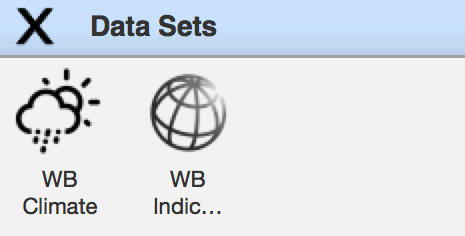
\includegraphics[width=4cm]{pic/data_sets_group.png}
  \end{center}
  \caption{Skupina gradnikov data sets}
  \label{data_sets_group}
\end{figure} 


\subsection{Gradnik WB Indicators}

\verb|WB Indicators| je gradnik programa Orange za dostop do podatkov
programskega vmesnika indikatorjev. Ta gradnik nam omogo"ca enastavno izbiro
enega ali ve"c indikatorjev in ene ali ve"c dr"zav za katere "zelimo dobiti
podatke izbranih indikatorjev. Za la"zje iskanje indikatorjev smo v grafi"cnem
vmesniku dodali dve mo"znosti presejanja seznama indikatorjev. Pri prvem situ
si lahko izberemo prikaz vseh indikatorjev, pogosto uporabljenih 
indikatorjev\footnote{Seznam je na voljo na strani 
\url{http://data.worldbank.org/indicator?tab=all}}
ali pa izpostavljenih indikatorjev\footnote{Seznam je na voljo na strani 
\url{http://data.worldbank.org/indicator?tab=featured}}. Drugo sit pa je
tekstovno presejanje po poljih: koda ``Id'', ime ``Name'', teme ``Topics'' in
viri ``Sources''. 
% TODO: preveri ta stavek
V grafi"cnem vmesniku si lahko tudi izberemo eno izmed oblik izhodnih podatkov
kot "casovne vrste \angl{Time Series} ali podatke dr"zav \angl{Countries}, 
kot smo ju opisali v razdelku \ref{razred_indicatordatasets}. 
Implementirali pa smo tudi prikaz napredka prenosa podatkov, s "stevili vseh in
"ze izvedenih poizveb, omenjeni v razdelku \ref{razered_indicator_api}.


\begin{figure}
\begin{center}
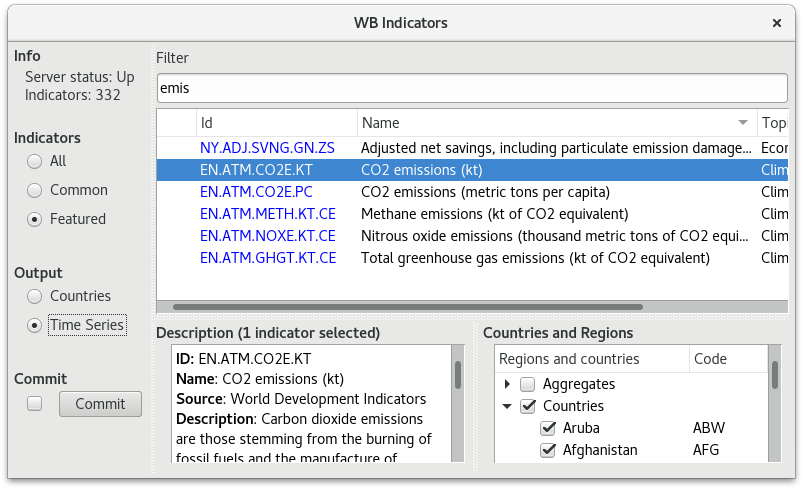
\includegraphics[width=12cm]{pic/co2_temp_indicator_selection.png}
\end{center}
\caption{Prikaz gradnika WB Indicators.}
\label{co2_temp_indicator}
\end{figure} 




\subsection{Gradnik WB Climate}

Gradnik za izbiro podnebnih podatkov podatkovnega vmesnika Svetovne banke, nam
ponuja mo"znosti izbire dr"zav, vrste podatkov in vrste meritvenega obdobja.
Prav tako kot gradnik WB Indicators, lahko tudi tukaj izberemo obliko izhodnih
podatkov. Mo"zni izbiri oblike izhodnih podatkov sta "casovne vrste in podatki
dr"zav, kot smo opisani v poglavju \ref{razsiritev_razreda_climatedataset}. 
Kot dodatno mo"znost pa imamo v tem grafi"cnem vmesniku tudi zastavico, ki 
dolo"ca ali bomo za dr"zave izpisovali imena ali pa kode. Tudi temu grafi"cnemu
vmesniku smo dodali prikaz napredka prenosa podatkov.



\begin{figure}
\begin{center}
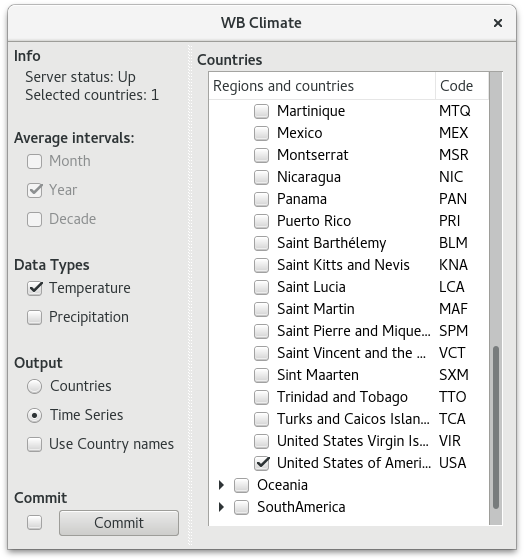
\includegraphics[width=12cm]{pic/co2_temp_climate_selection.png}
\end{center}
\caption{Prikaz gradnika WB Climate.}
\label{co2_temp_climate}
\end{figure} 

\chapter{Primeri uporabe}


\section{Uporaba modula api\_wrapper}

Enostavno uporabo modula \verb|api_wrapper| s skriptnim delom programa Orange
prikazuje primer \ref{scripting_example}. V temu primeru pogledamo, kako
učinkovito lahko napovemo smrtnost otrok iz raznih indikatorjev zdravja,
okolja in infrastrukture. V vrsticah $5$ do $15$ naredimo poizvedbe po
potrebnih podatkih s programskega vmesnika Svetovne banke. Nato v vrsticah $18$
do $27$ odstranimo vrstice iz tabele, ki nimajo ciljne vrednosti in naredimo novo tabelo z
razredom, ki ga želimo napovedovati. Vrednosti, ki jih želimo napovedovati, se
nahajajo v stolpcu $55$ v tabeli \verb|class_data|. Ta stolpec vsebuje podatke
o smrtnosti otrok mlajših od enega leta za leto 2015. V naslednjih vrsticah
pa zgradimo tri napovedne modele: naključni gozd z
regresijskimi drevesi \verb|rf|, linearna regresija z regularizacijo 
\verb|ridge| in srednja vrednost \verb|mean|.
Za ocene napovednih modelov smo uporabili oceni
$RMSE$~\fnurl{https://en.wikipedia.org/wiki/Root-mean-square\_deviation} in 
$R^2$~\fnurl{https://en.wikipedia.org/wiki/Coefficient\_of\_determination}.
Rezultate primera \ref{scripting_example} lahko vidimo v tabeli 
\ref{rezultati_skripte}.


\begin{snippet}
\begin{center}
\lstinputlisting{example.py}
\end{center}
\cprotect
\caption{Napovedovanje smrtnosti otrok do enega leta iz podatkov o dostopnosti
  čiste vode, številu bolniških postelj na 1000 prebivalcev in odstotku
  cepljenih otrok do drugega leta starosti.}
\label{scripting_example}
\end{snippet} 

\begin{table}
\begin{center}

\begin{tabular}{l|r|r}
  Learner & RMSE & R2 \\ \hline
  rf & 9.74 & 0.79 \\
  ridge & 17.76 & 0.31 \\
  mean & 21.35 & -0.00
\end{tabular}
\end{center}
\cprotect
\caption{Rezultati napovedi smrtnosti otrok do enega leta starosti.}
\label{rezultati_skripte}
\end{table} 



\section{Napoved temperature s pomočjo $CO_2$ izpustov v ZDA}


Podatke svetovne banke lahko uporabimo tudi kot časovne vrste z uporabo
posebnih gradnikov za delo s časovnimi vrstami \cite{time_series}. Tukaj si
bomo ogledali enostaven primer napovedi temperature v ZDA s pomočjo podatkov o
izpustih $CO_2$. V tej napovedi smo uporabili podatke tako z gradnika 
WB Indicators (Slika \ref{var_indicator_select})
kot tudi z gradnika WB Climate (Slika \ref{var_climate_select}). Podatke obeh
gradnikov smo zdru"zili z gradnikom ``Merge Data'' po obeh "casovnih
komponentah. Nato smo odstranili vnose "casovnih obdobij za katere nimamo na
voljo vseh podatkov. Sestavljeno tabelo prikazuje slika \ref{var_data_table}.
Iz teh podatkov nato zgradimo "casovno vrsto in s pomočjo modela vektorske 
autoregresije VAR \cite{var_model} napovemo podatke za povprečno 
letno temperaturo za naslednjih nekaj let, kar je prikazano na sliki 
\ref{var_forecast_graph}.

\begin{figure}
\begin{center}
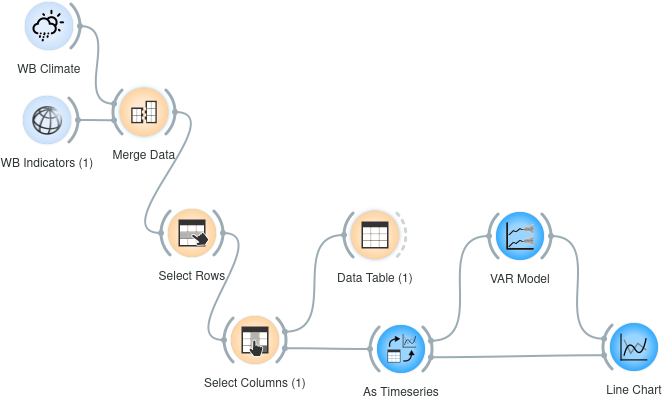
\includegraphics[width=11cm]{pic/var_setup.png}
\end{center}
\caption{Prikaz povezave gradnikov za napoved temperature.}
\label{var_setup}
\end{figure} 


\begin{figure}
\begin{center}
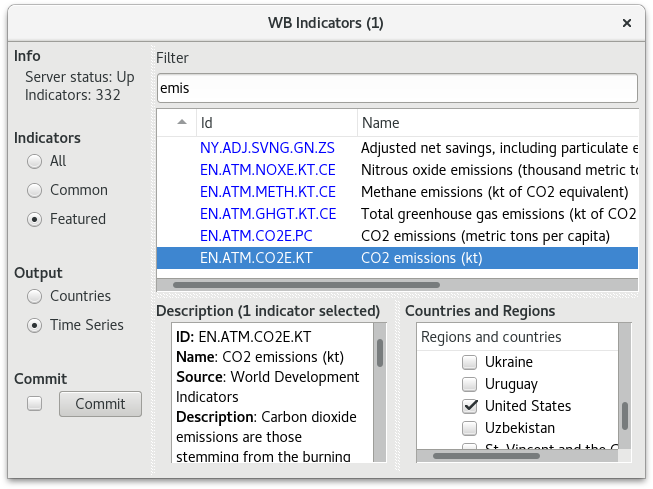
\includegraphics[width=12cm]{pic/var_indicator_select.png}
\end{center}
\caption{Izbor indikatorja $CO_2$ izpustov v ZDA.}
\label{var_indicator_select}
\end{figure} 

\begin{figure}
\begin{center}
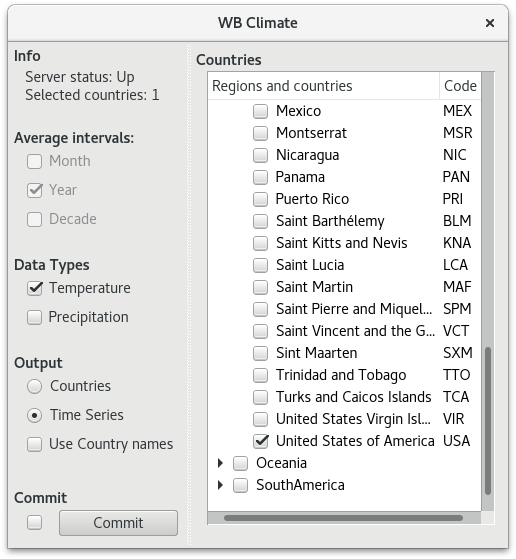
\includegraphics[width=8cm]{pic/var_climate_select.png}
\end{center}
\caption{Izbor podatkov povprečnih letnih temperatur v ZDA.}
\label{var_climate_select}
\end{figure} 

\begin{figure}
\begin{center}
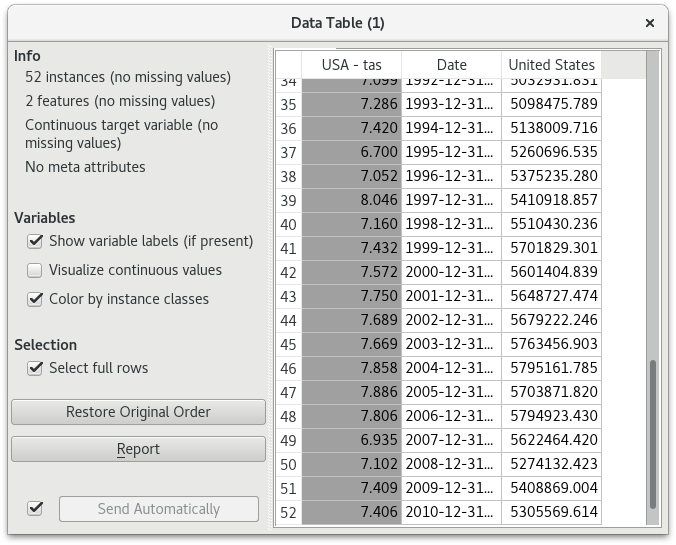
\includegraphics[width=10cm]{pic/var_data_table.png}
\end{center}
\caption{Podatkovna tabela s ciljnim razredom, in dvema poljema.}
\label{var_data_table}
\end{figure} 

\begin{figure}
\begin{center}
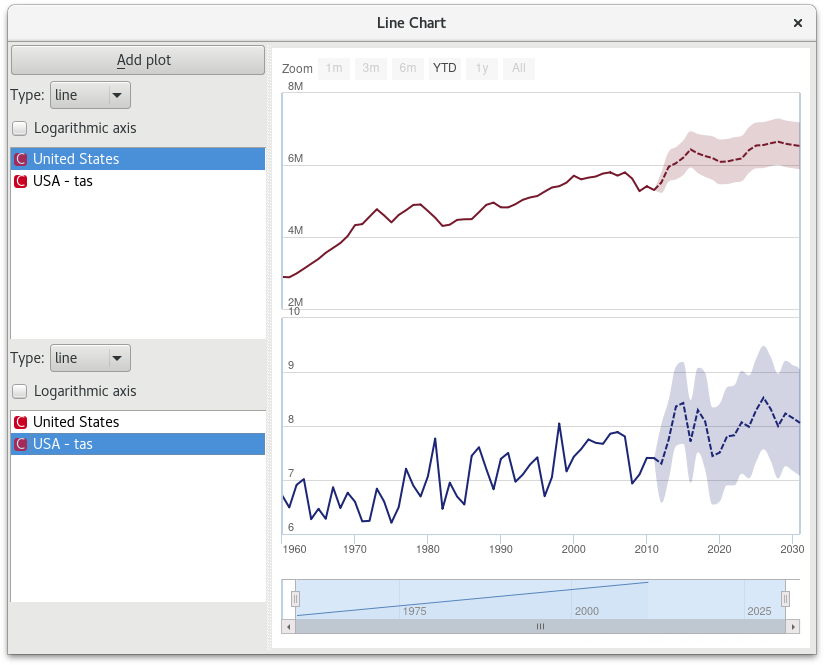
\includegraphics[width=12cm]{pic/var_forecast_graph.png}
\end{center}
\caption{Prikaz napovedi gibanja povprečnih letnih temperatur ``USA - tas'' in
  $CO_2$ izpustov ``United States''.}
\label{var_forecast_graph}
\end{figure} 




\section{Gru"cenje dr"zav}


Podatke, ki jih dobimo z na"sim dodatkom, lahko v programu Orange uporabimo tudi
za grafi"cni prikaz statistik in povezav med dr"zavami. Kot mo"zen primer
uporabe (Slika \ref{clustering_setup}) smo prikazali gru"cenje dr"zav svetovnih regij glede na naslednje
indikatorje (Slika \ref{clustering_indicator_selection}):
\begin{itemize}
  \item odstotek ljudi ki "zivijo v urbanem okolju 
    \angl{Urban population (\% of total)},
  \item smrtnost na $1000$ "zivorojenih otrok
    \angl{Mortality rate, infant (per 1,000 live births)},
  \item "stevilo bolni"skih postelj na $1000$ prebivalcev
    \angl{Hospital beds (per 1,000 people)},
  \item odstotek BDP izdatkov za raziskave in razvoj
    \angl{Research and development expenditure (\% of GDP)},
  \item "stevilo prebivalstva pod pragom rev"s"cine pri meji $3.10$ dolarjev na dan
    \angl{Poverty gap at $\$3.10$ a day (2011 PPP) (\%)}.
\end{itemize}
Med temi indikatorji smo izra"cunali evklidsko razdaljo in za prikaz 
uporabili "ze obstoje"ca gradnika programa Orange
``MDS'' (slika \ref{clustering_mds}) in
``Hierarchical Clustering'' (slika \ref{clustering_hierarchial_countries}).



\angl{multidimensional scaling}. 
% ID: SP.URB.TOTL.IN.ZS 
% Name:  
% ID: SP.DYN.IMRT.IN 
% Name:  
% ID: SI.POV.GAP2 
% Name: 
% ID: SH.MED.BEDS.ZS 
% Name: 
% ID: GB.XPD.RSDV.GD.ZS 
% Name: 


\begin{figure}
\begin{center}
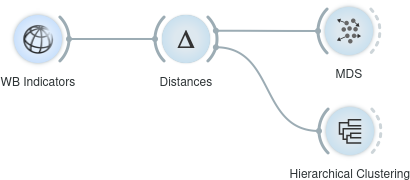
\includegraphics[width=5cm]{pic/clustering_setup.png}
\end{center}
\caption{Postavitev okolja za prikaz gru"cenja.}
\label{clustering_setup}
\end{figure} 

\begin{figure}
\begin{center}
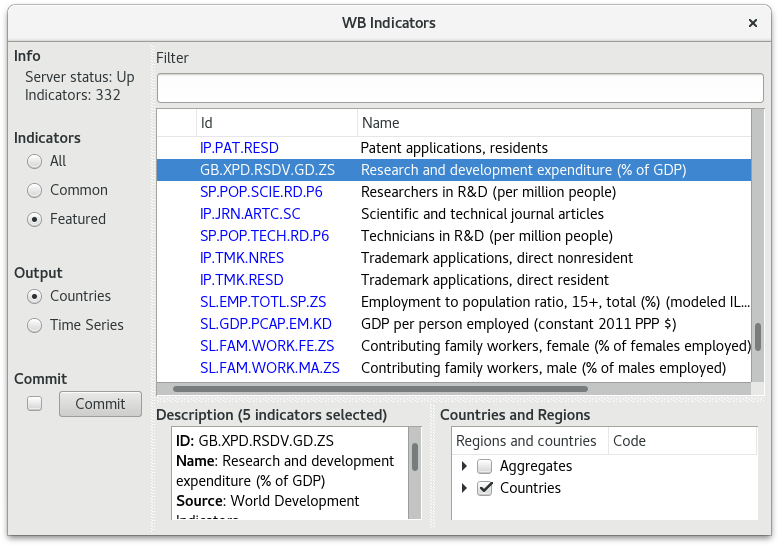
\includegraphics[width=12cm]{pic/clustering_indicator_selection.png}
\end{center}
\caption{Izbor indikatorjev za gru"cenje.}
\label{clustering_indicator_selection}
\end{figure} 

\begin{figure}
\begin{center}
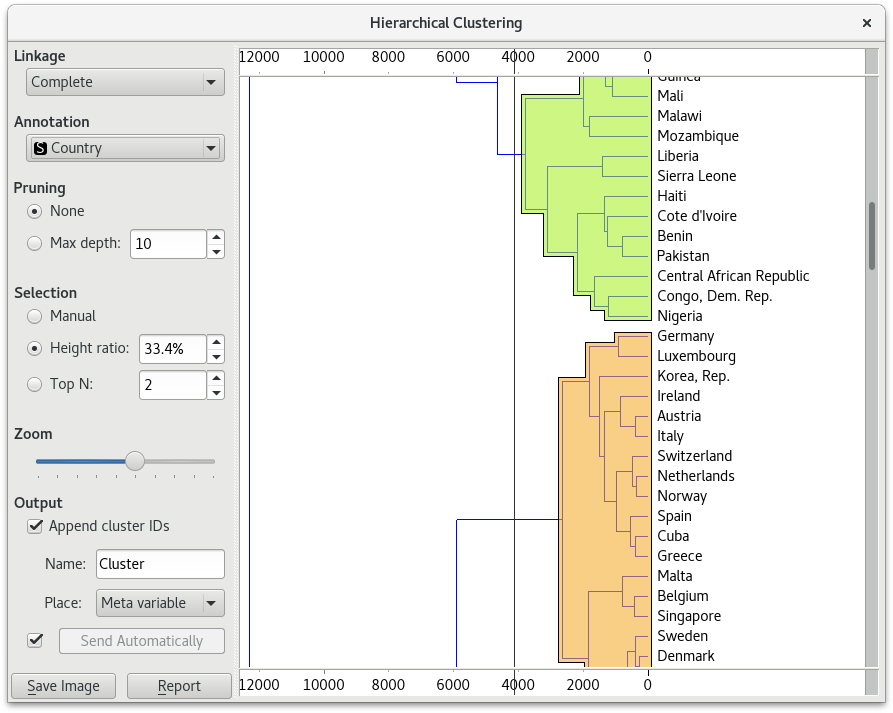
\includegraphics[width=12cm]{pic/clustering_hierarchial_countries.png}
\end{center}
\caption{Prikaz hierarhi"cnega gru"cenja dr"zav.}
\label{clustering_hierarchial_countries}
\end{figure} 

\begin{figure}
\begin{center}
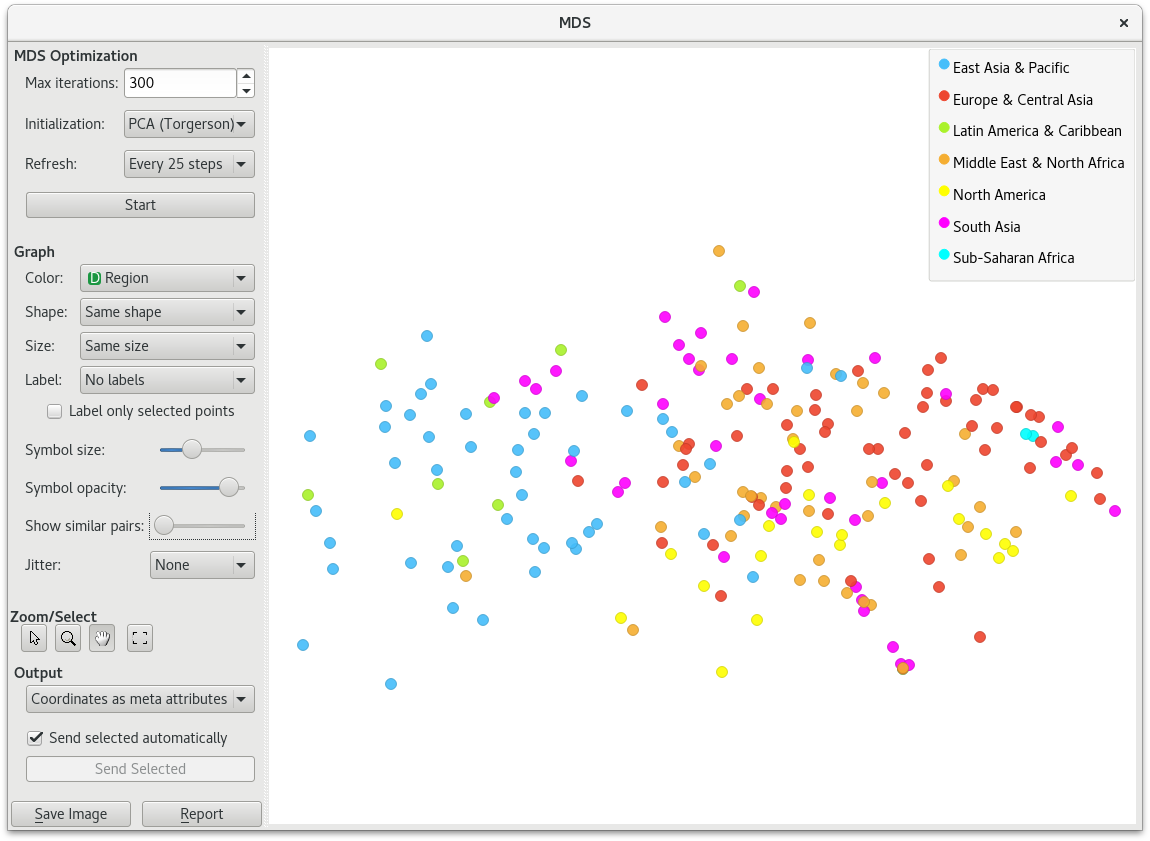
\includegraphics[width=12cm]{pic/clustering_mds.png}
\end{center}
\caption{Prikaz gru"cenja MDS.}
\label{clustering_mds}
\end{figure} 


\chapter{Sklepne ugotovitve}


% zaključek (odstavki: kaj smo naredili in kje je koda, kaj nam to omogoča, 
% kaj bi lahko še naredili)

Z izdelavo dodatka za program Orange smo zakljucili delo na diplomski nalogi.
Koda izdelanega dodatka se nahaja na git ....


% S tem dodatkom smo omogo"cili dostop do podatkov Svetovne banke tudi
% uporabnikom programa Orange brez znanja o samem programskem vmesniku SB.
% 
% S tem dodatkom smo olajsali dostop do velike zbirke podatkov Svetovne banke,
% ki jih lahko sedaj znotraj programa Orange za svoje delo uporabi kdorkoli.
%
%- lazje vzdrzevanje in posodabljanje kode
%
%
%
%Tako smo omogo"cili lazje


Nas grafi"cni dodatek za dostop do podatkov indikatorjev lahko nadgradimo tako,
da uporabnikom grafi"cnega vmesnika omogo"cimo ve"cjo izbiro oblik izhodnih
podatkov in natan"cnejse presejanje rezultatov. Dodamo lahko tudi ve"c
metapodatkov na posamezne stolpce Orange tabele, ki nam omogo"cijo bolj"so
predstavnost v ostalih Orange gradnikih. V grafi"cni vmesnik za dostop do
podnebnih podatkov lahko dodamo "se mo"znost izbire vodoto"cnih obmo"cji meritev.
Za bolj"so predstavo bi lahko postopek izbire drzav, regij in vodoto"cnih
obmo"cij omogo"cili prek interaktivnega zemljevida sveta.


- dodamo metapodatke tudi climate gradniku
- boljsa pokritost testov

\begin{thebibliography}{1}

% Indicator data sources

\bibitem{world_dev_ind} World Development Indicators, The World Bank, (August 2016)
\\ URL: \url{http://data.worldbank.org/data-catalog/world-development-indicators}

\bibitem{glob_fin_dev} Data source: Global Financial Development Database (GFDD), The World Bank. Methodology citation: Martin Čihák, Aslı Demirgüç-Kunt, Erik Feyen, and Ross Levine, 2012. ``Benchmarking Financial Systems Around the World.'' World Bank Policy Research Working Paper 6175, World Bank, Washington, D.C. (Junij 2016)
\\ \url{http://data.worldbank.org/data-catalog/global-financial-development}

% \bibitem{int_debt_stat} International Debt Statistics, The World Bank (December 2015) 
% \\ \url{http://data.worldbank.org/data-catalog/international-debt-statistics}

\bibitem{africa_dev_ind} Africa Development Indicators, The World Bank (Februar 2013)
\\ \url{http://data.worldbank.org/data-catalog/africa-development-indicators}

\bibitem{doing_buseness} Doing Business, The World Bank (http://www.doingbusiness.org) (Julij 2016)
\\ \url{http://data.worldbank.org/data-catalog/doing-business-database}

\bibitem{ent_surveys} Enterprise Surveys, The World Bank (Julij 2016)
\\ \url{http://data.worldbank.org/data-catalog/enterprise-surveys}

\bibitem{mil_dev_goals} Millennium Development Goals, The World Bank (Julij 2016)
\\ \url{http://data.worldbank.org/data-catalog/millennium-development-indicators}

\bibitem{edu_stat} World Bank EdStats (Junij 2016)
\\ \url{http://data.worldbank.org/data-catalog/ed-stats}

\bibitem{gen_stat} Gender Statistics, The World Bank (Julij 2016)
\\ \url{http://data.worldbank.org/data-catalog/gender-statistics}

\bibitem{health_pop_stat} HealthStats, World Bank Group (Julij 2016)
\\ \url{http://data.worldbank.org/data-catalog/health-nutrition-and-population-statistics}

\bibitem{ida_res_mes_sys} IDA Results Measurement System, the World Bank (Julij 2016)
\\ \url{http://data.worldbank.org/data-catalog/IDA-results-measurement}

\bibitem{climate_data} Climatic Research Unit, University of East Anglia
\\ \url{http://www.cru.uea.ac.uk/data}

\bibitem{orange_scripting} Janez Demšar and Tomaž Curk and Aleš Erjavec and Črt Gorup and Tomaž Hočevar and Mitar Milutinovič and Martin Možina and Matija Polajnar and Marko Toplak and Anže Starič and Miha Štajdohar and Lan Umek and Lan Žagar and Jure Žbontar and Marinka Žitnik and Blaž Zupan, ``Orange: Data Mining Toolbox in Python,'' Journal of Machine Learning Research, vol. 14, pp. 2349-2353, 2013.


\bibitem{time_series} Jernej Kernc, ``Orodje za interaktivno analizo časovnih vrst,'' 2016


\bibitem{var_model}  Eric Zivot, Jiahui Wang, ``Vector Autoregressive Models for Multivariate Time Series'' Modeling Financial Time Series with S-PLUS, pp. 385-429, 2006.






\bibitem{jezicno} Jure Dimec (2002), Medjezično iskanje dokumentov 
\\ \url{http://clir.craynaud.com/clir/MEDJEZICNOISKANJEDOKUMENTOV.pdf}


% \bibitem{opengl} (Avgust, 2013) OpenGL Overview
% \\ \url{http://www.opengl.org/about/}

\end{thebibliography}


%\begin{thebibliography}{99}
%\bibitem{lf} L.\ Fortnow, ``Viewpoint: Time for computer science to grow up'',
%{\it Communications of the ACM}, št.\ 52, zv.\ 8, str.\ 33--35, 2009.
%\bibitem{dk1} D.\ E.\ Knuth, P. Bendix. ``Simple word problems in universal algebras'', v zborniku: Computational Problems in Abstract Algebra (ur. J. Leech), 1970, str. 263--297.
%\bibitem{lat} L.\ Lamport. {\it LaTEX: A Document Preparation System}. Addison-Wesley, 1986.
%\bibitem{bib} O.\ Patashnik (1998) \BibTeX{}ing. 
%\\ http://ftp.univie.ac.at/packages/tex/biblio/bibtex/contrib/doc/btxdoc.pdf
%\bibitem{licence} licence-cc.pdf. Dostopno na: 
%\end{thebibliography}



\end{document}

